\chapter{Interfaz Hardware - Software}
\label{capituloInterfaz}
\par La interfaz de comunicación entre la estación de recolección y el software (aplicación móvil) debe permitir que los datos recolectados por la primera sean transmitidos hacia la aplicación de manera coherente. La aplicación, por su parte, es la encargada de procesar los datos y enviar las señales correspondientes de vuelta al Raspberry\textsuperscript{\textregistered}.
\par En este capítulo se presenta y justifica la tecnología utilizada, el diseño concebido, y finalmente, el desarrollo del componente.

    \section{Análisis de alternativas}
    \par A continuación se presentan las alternativas analizadas durante el proceso de elección de tecnologías para este componente.
        \subsection{Alternativas}
            \subsubsection{Tecnologías alámbricas}
                \par La utilización de esta tecnología proporciona una comunicación robusta respecto a los ruidos que producen motores y artefactos en funcionamiento, elementos frecuentemente presentes en fábricas, que pueden producir alteraciones de los datos transmitidos. Además, se asegura la conexión punto a punto libre de pérdidas de conexión que se pueden producir en tecnologías inalámbricas.
                
                \par El diseño de este sistema incorpora el uso de un dispositivo móvil, el cual utiliza una conexión cableada de tipo USB como opción única para su conexión alámbrica. Según el estándar USB\footnote{Página oficial del estándar USB: \url{https://usb.org}}, la especificación de su funcionamiento se limita a una longitud máxima de 5 metros usando su versión de conexión USB 2.0.
                
                \par En consecuencia a lo antes mencionado, ubicándose espacialmente en una planta de producción de tamaño pequeño a mediano, esta opción presenta un evidente entorpecimiento al momento de operar el equipo  y/o desplazarse por ella. El productor en su accionar lleva adelante distintas tareas en simultaneo realizando preparativos para los distintas etapas del proceso, mediante la utilización de una conexión cableada y de longitud limitada esta operatoria es afectada negativamente.
                
            \subsubsection{Tecnologías inalámbricas}
                \par Los estándares más utilizados dentro de esta tecnología son: Wi-Fi\textsuperscript{\textregistered} (IEEE\footnote{ \textit{Institute of Electrical and Electronics Engineers}, Instituto de Ingeniería Eléctrica y Electrónica} 802.11x) y Bluetooth\textsuperscript{\textregistered} (IEEE 802.15x).
                \paragraph{Wi-Fi\textsuperscript{\textregistered}:} Es una marca comercial de Wi-Fi Alliance (una organización que adopta y certifica los equipos que cumplen con los estándares 802.11 de las redes inalámbricas de área local). El objetivo tras la marca Wi-Fi\textsuperscript{\textregistered} es fomentar las conexiones inalámbricas y facilitar la compatibilidad de los distintos equipos. Esta tecnología permite la comunicación de datos entre un dispositivo y todos aquellos que se encuentren dentro del área de cobertura del mismo o de la red de un punto de acceso al que se encuentre conectado este. Para ello utiliza enlace de radio frecuencia de 2.4, 3.6 o 5Ghz, dependiendo el estándar que se utilice.
                \paragraph{Bluetooth\textsuperscript{\textregistered}:} Bluetooth\textsuperscript{\textregistered} es una especificación industrial para Redes Inalámbricas de Área Personal (WPAN) creado por Bluetooth Special Interest Group, Inc. que posibilita la transmisión de voz y datos entre diferentes dispositivos mediante un enlace por radiofrecuencia en la banda ISM de los 2.4 GHz.
                
                \par En el Anexo \ref{tab:ComparacionInterfaz} se ubica una tabla comparativa entre ambas tecnologías. Se utilizan como criterios de comparación aquellos relevantes para la realización de este proyecto. 
        
        \subsection{Tecnologías utilizadas}
            \par Dadas las limitaciones y consecuencias aparejadas del uso de una tecnología alámbrica a ser incorporada en el presente diseño, se opta por el uso de tecnología inalámbrica dadas las ventajas que las mismas aportan al diseño del presente sistema. De esta manera, con una conexión inalámbrica, el productor puede desplazarse con su dispositivo móvil con total libertad durante el transcurso del proceso, sin dejar de realizar el seguimiento con el dispositivo.
            
            \par Dado el tamaño del equipo productivo de los usuarios para los que este sistema es destinado, no se presentan maquinarias que pudiesen ocasionar ruido al canal inalámbrico de comunicación. Por tanto, un análisis de ruido en los canales de comunicación carece de relevancia para este sistema. Sin embargo, se prevé el desarrollo de un protocolo de comunicación capaz de recuperar datos ante intermitencia en la comunicación entre las partes involucradas, la estación de recolección de datos y el dispositivo móvil. 
            
            \par A partir de los datos comparados de la Tabla \ref{tab:ComparacionInterfaz} ubicada en el Anexo, se opta por utilizar la tecnología WiFi\textsuperscript{\textregistered}. Esto se basa en su rango de conexión y la cantidad de dispositivos conectados que permite. A partir de la elección de esta tecnología de comunicación inalámbrica, se define instalar un servidor web que opere sobre el componente electrónico y, posteriormente, un servicio web REST API \footnote{REST API, representational state transfer (REST) application program interface (API), es una interfaz que utiliza requerimientos HTTP tipo GET, PUT, POST and DELETE para transferencia de datos.}, funcionando en este contexto, que permita establecer una comunicación entre el dispositivo móvil y el componente electrónico. Dadas las recomendaciones del fabricante del componente electrónico, la multiplicidad de guías, comunidad y soporte, se opta por la utilización de la tecnología Apache para la instalación del servidor web. A partir de esta elección, se propone PHP\footnote{PHP (acrónimo recursivo de PHP: Hypertext Preprocessor) es un lenguaje de código abierto muy popular especialmente adecuado para el desarrollo web.} como tecnología de desarrollo por cuestiones de agilidad y coexistencia.
    %%        
    \section{Diseño}
    A continuación, se describen las consideraciones previas al proceso de diseño de la interfaz, luego se presenta el resultado de este diseño.
        
        \subsection{Consideraciones previas}
            \par En este apartado se describen distintas restricciones inherentes al funcionamiento del sistema que se consideraron para el diseño del mismo. Cada una será descrita con el fin de fundamentar la decisión de diseño elegida.

            \paragraph{Capacidad de ejecutar código Python:}
                \par Los scripts para obtención y almacenamiento de mediciones fueron escritos en lenguaje Python. Por esto, la REST API  debe poder ejecutar este tipo de archivos. Las llamadas de ejecución deben permitir adjuntar parámetros de configuración.
        
            \paragraph{Capacidad de establecer conexión con la base de datos:} 
                \par La REST API debe poder conectarse a la base de datos alojada en el servidor para realizar lectura y escritura de datos.
       
            \paragraph{Capacidad de ejecutar distintas funcionalidades en forma paralela:}
                \par Es requisito del sistema ejecutar de manera simultánea y continua la transmisión de datos entre el componente de hardware y software mientras se procede con la recolección de datos de la experiencia.
            
            \paragraph{Capacidad de mantener la coherencia de datos:}
                \par La detección de una falla durante el experimento es realizada por el componente de software. Por ende, la interfaz debe ofrecer la posibilidad de eliminar los datos corruptos correspondientes a una maceración inconclusa de la base de datos, alojada en el componente electrónico, con el fin de mantener la coherencia de los datos.
            
        
        
        \subsection{Diseño de la interfaz}
        %\hfill \break
        %\begin{minipage}{\textwidth} 
            \par En cuanto al diseño de la REST API, se opta por codificar cada funcionalidad en un archivo independiente y cumplir de esta manera con la consideración previa de ejecución paralela.
            \par En la Tabla \ref{tab:FuncionalidadesInterfaz} se presenta una descripción de funcionalidades:
            
            
            
            
            \begin{longtable}{|p{2.2cm}|p{4.8cm}|p{3.5cm}|p{3.5cm}|}
            \hline
            \multicolumn{4}{| c |}{\textbf{Tabla de funcionalidades de la interfaz}}\\
            \hline
            \multicolumn{1}{| c |}{Nombre} &\multicolumn{1}{| c |}{Funcionalidad} & \multicolumn{1}{| c |}{Retorno} &\multicolumn{1}{| c |}{Parámetros}\\
           
            \hline
            \hline
            \endfirsthead
            
            \hline
            \multicolumn{4}{|c|}{Continuación de la Tabla \ref{tab:FuncionalidadesInterfaz}}\\
            \hline
             \multicolumn{1}{| c |}{Nombre} &\multicolumn{1}{| c |}{Funcionalidad} & \multicolumn{1}{| c |}{Retorno} &\multicolumn{1}{| c |}{Parámetros}\\
            \hline
            \endhead
            
            \endfoot
 
            \caption{Descripción de funcionalidades de la interfaz Hardware - Software \label{tab:FuncionalidadesInterfaz}}\\
            \endlastfoot
             
            Inicio de experimento de maceración & Inserta en la base de datos la maceración (en caso de ser una nueva entrada) y el experimento. Ejecuta los archivos Python utilizando como parámetros la duración del experimento y los intervalos de medición. & & Nombre maceración,  duración, intervalos de medición de temperatura y pH, e ID de experimento. \\ 
            \hline
            
            Obtención de valores recolectados de un experimento de maceración & A partir de un ID de experimento y una lista de valores recolectados (obtenidos previamente por la aplicación), la REST API consulta la base de datos y retorna las mediciones correspondientes a cada ID de experimento no presente en el conjunto enviado. & Arreglo de medidas por experimento. Número N de conjuntos de: Medidas de temperatura del líquido; pH; temperatura y humedad ambiente & ID experimento, lista de valores recolectados obtenidos en consultas anteriores. \\ 
            \hline
                    
            Obtención de datos de sensores & 
            El componente de software (previsto a desarrollarse en las siguientes etapas) permite visualizar los valores actuales de los sensores. La funcionalidad encargada de acción ejecuta una rutina Python y retorna los valores a través de la REST API. & Medidas de temperatura del líquido; pH; temperatura y humedad ambiente. & \\
            \hline
                    
            Eliminación de un experimento de maceración & Eliminar el experimento y todos los datos recolectados que posean el ID de experimento pasado como parámetro. &  & ID experimento.\\
            \hline
                    
            Cancelación de un experimento de maceración & Detiene la ejecución de la librería Python, elimina los valores recolectados relacionados al ID de experimento y finalmente elimina el experimento mismo. & & ID experimento\\
            \hline
            
\end{longtable}     
  
    \section{Implementación del componente}
        \par En esta sección se describe el funcionamiento de la REST API desarrollada mediante diagramas de flujo de cada funcionalidad.
        
        \subsection{Inicio de experimento de maceración}
        \par En la Figura \ref{fig:ApiNuevoExp} se presenta el diagrama correspondiente a la API ``\textit{NuevoExp.php}''. Esta realiza la inserción de una nueva maceración y de un experimento. A continuación inicia el proceso de recolección de datos.
            \begin{figure}
                \centering
                %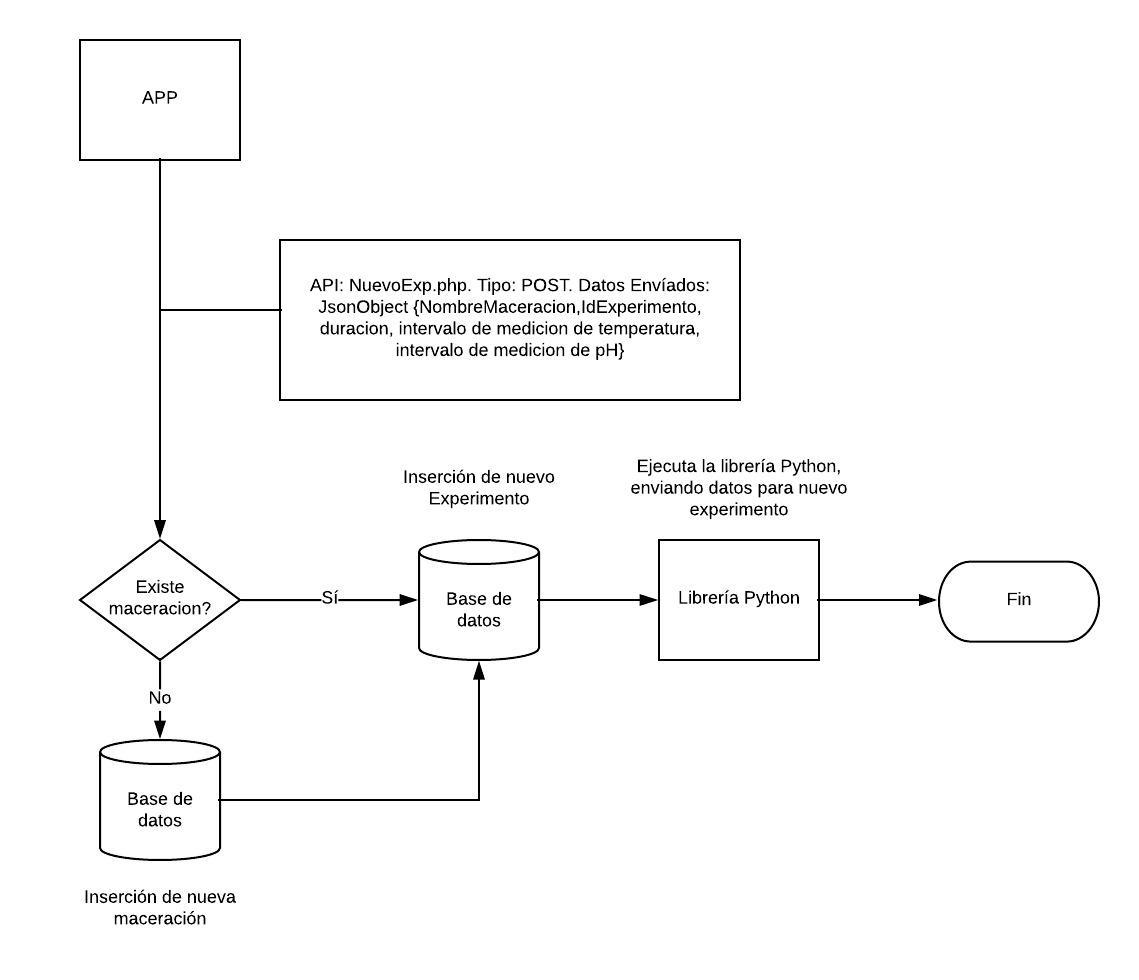
\includegraphics[scale=0.85]{DiagramaNuevoExp.jpeg}
                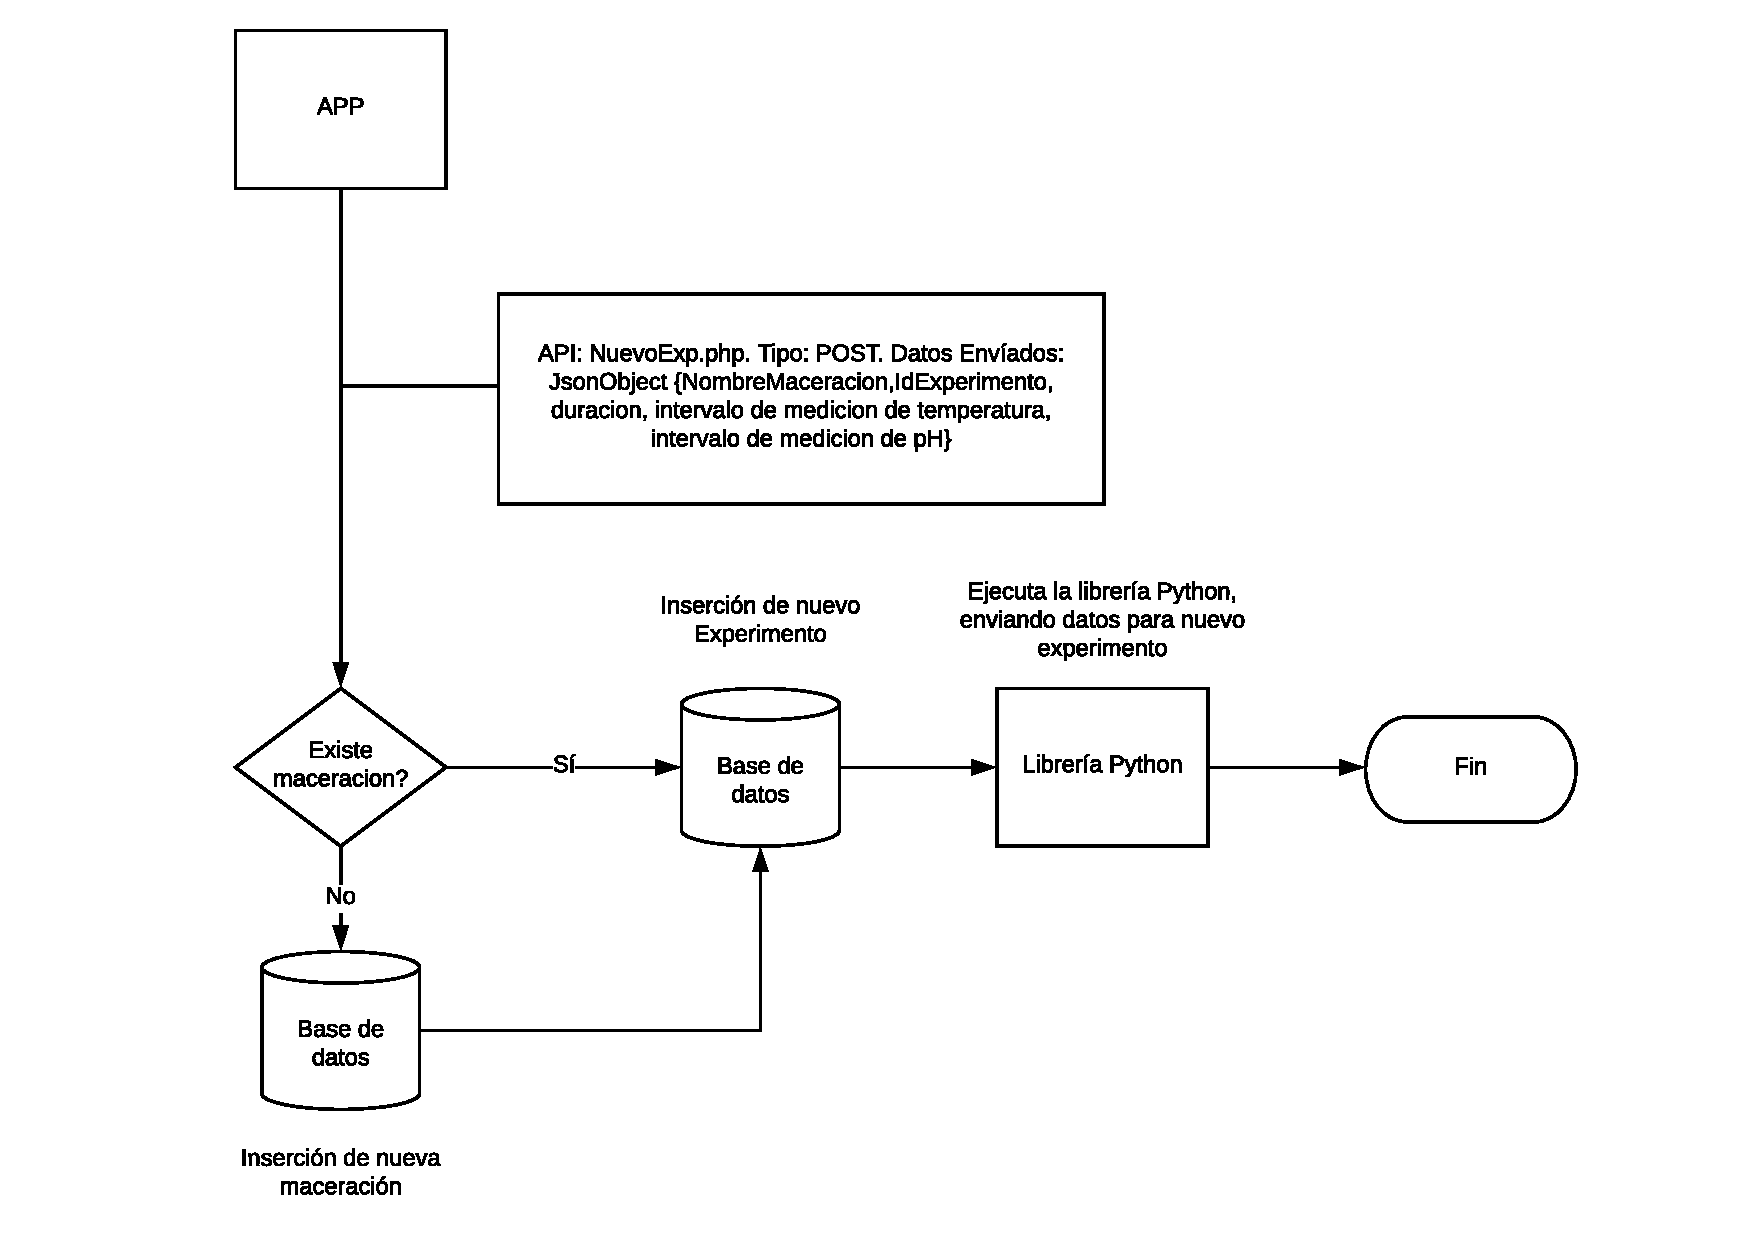
\includegraphics[scale=0.95]{Interfaz_Hard-Soft/DiagramaNuevoExp.pdf}
                \caption{Diagrama de flujo para nuevo experimento}
                \label{fig:ApiNuevoExp}
            \end{figure}
            
        \subsection{Obtención de valores recolectados de un experimento de maceración}
        
        \par En la Figura \ref{fig:ApiGet}, se presenta el diagrama correspondiente a la API ``\textit{ObtenerSensedValues.php}''. Esta es responsable de la obtención de nuevos conjuntos de valores recolectados relacionados a un ID de experimento particular, y su posterior envío a la aplicación móvil.
            \begin{figure}[h]
                \centering
                %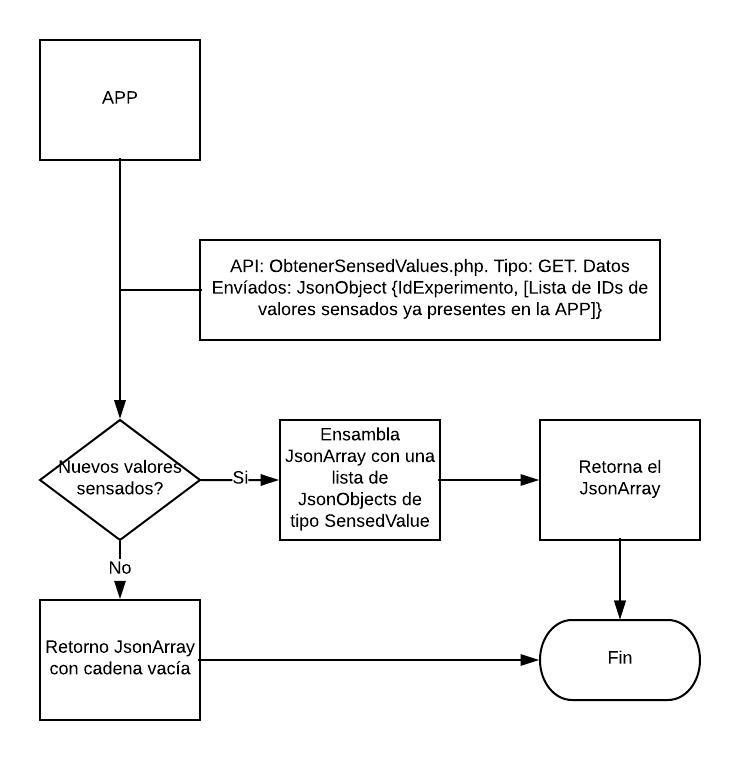
\includegraphics{DiagramaAPIGet.jpeg}
                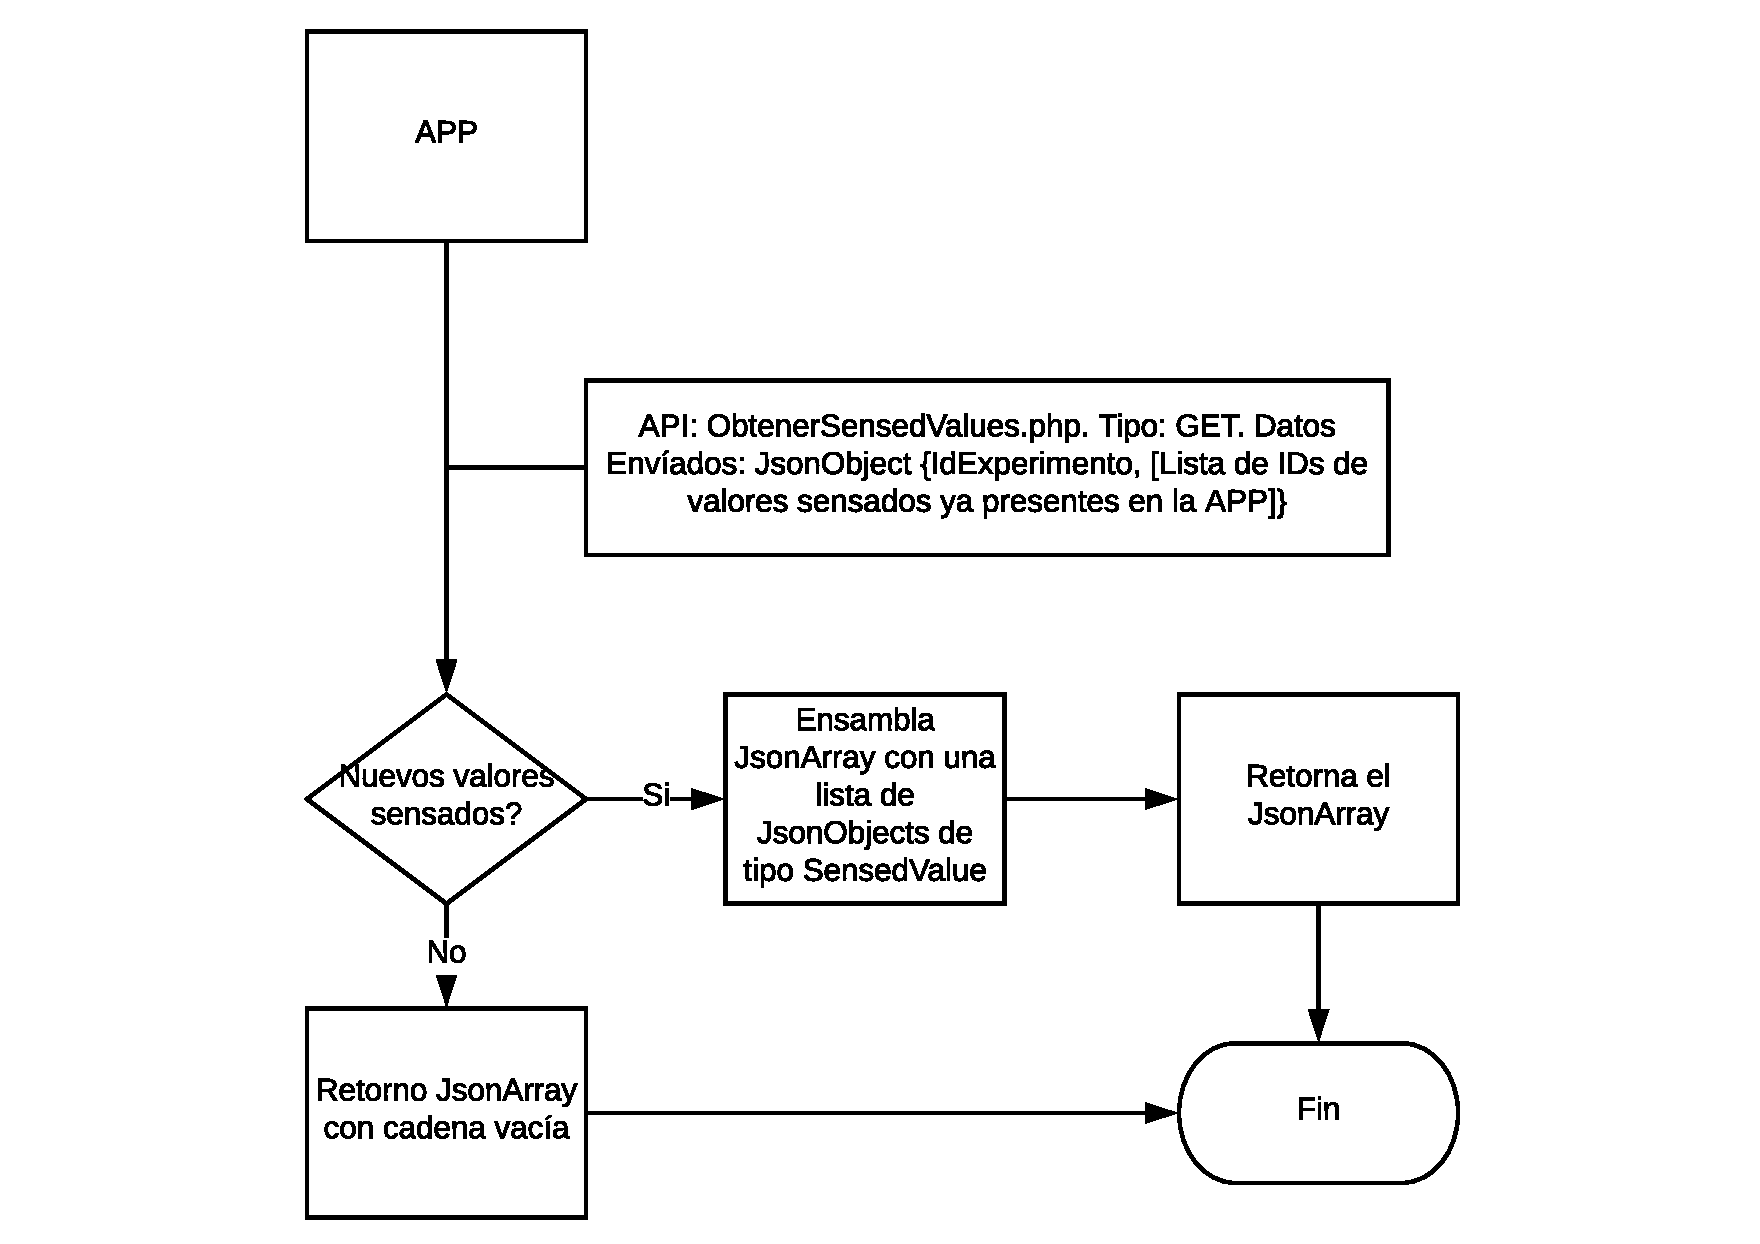
\includegraphics [scale=0.5] {DiagramaAPIGet.pdf}
                \caption{Diagrama de flujo para la obtención de valores sensados}
                \label{fig:ApiGet}
            \end{figure}
        
        \subsection{Obtención de datos de sensores}
        \par La API ``\textit{ObtenerMedicionActual.php}'', es responsable de la obtención de nuevos conjuntos de valores recolectados relacionados a un ID de experimento particular, y su posterior envío a la aplicación móvil. El diagrama de la misma se visualiza en la Figura \ref{fig:ApiGetTempPh}
        
            \begin{figure}[h]
                \centering
                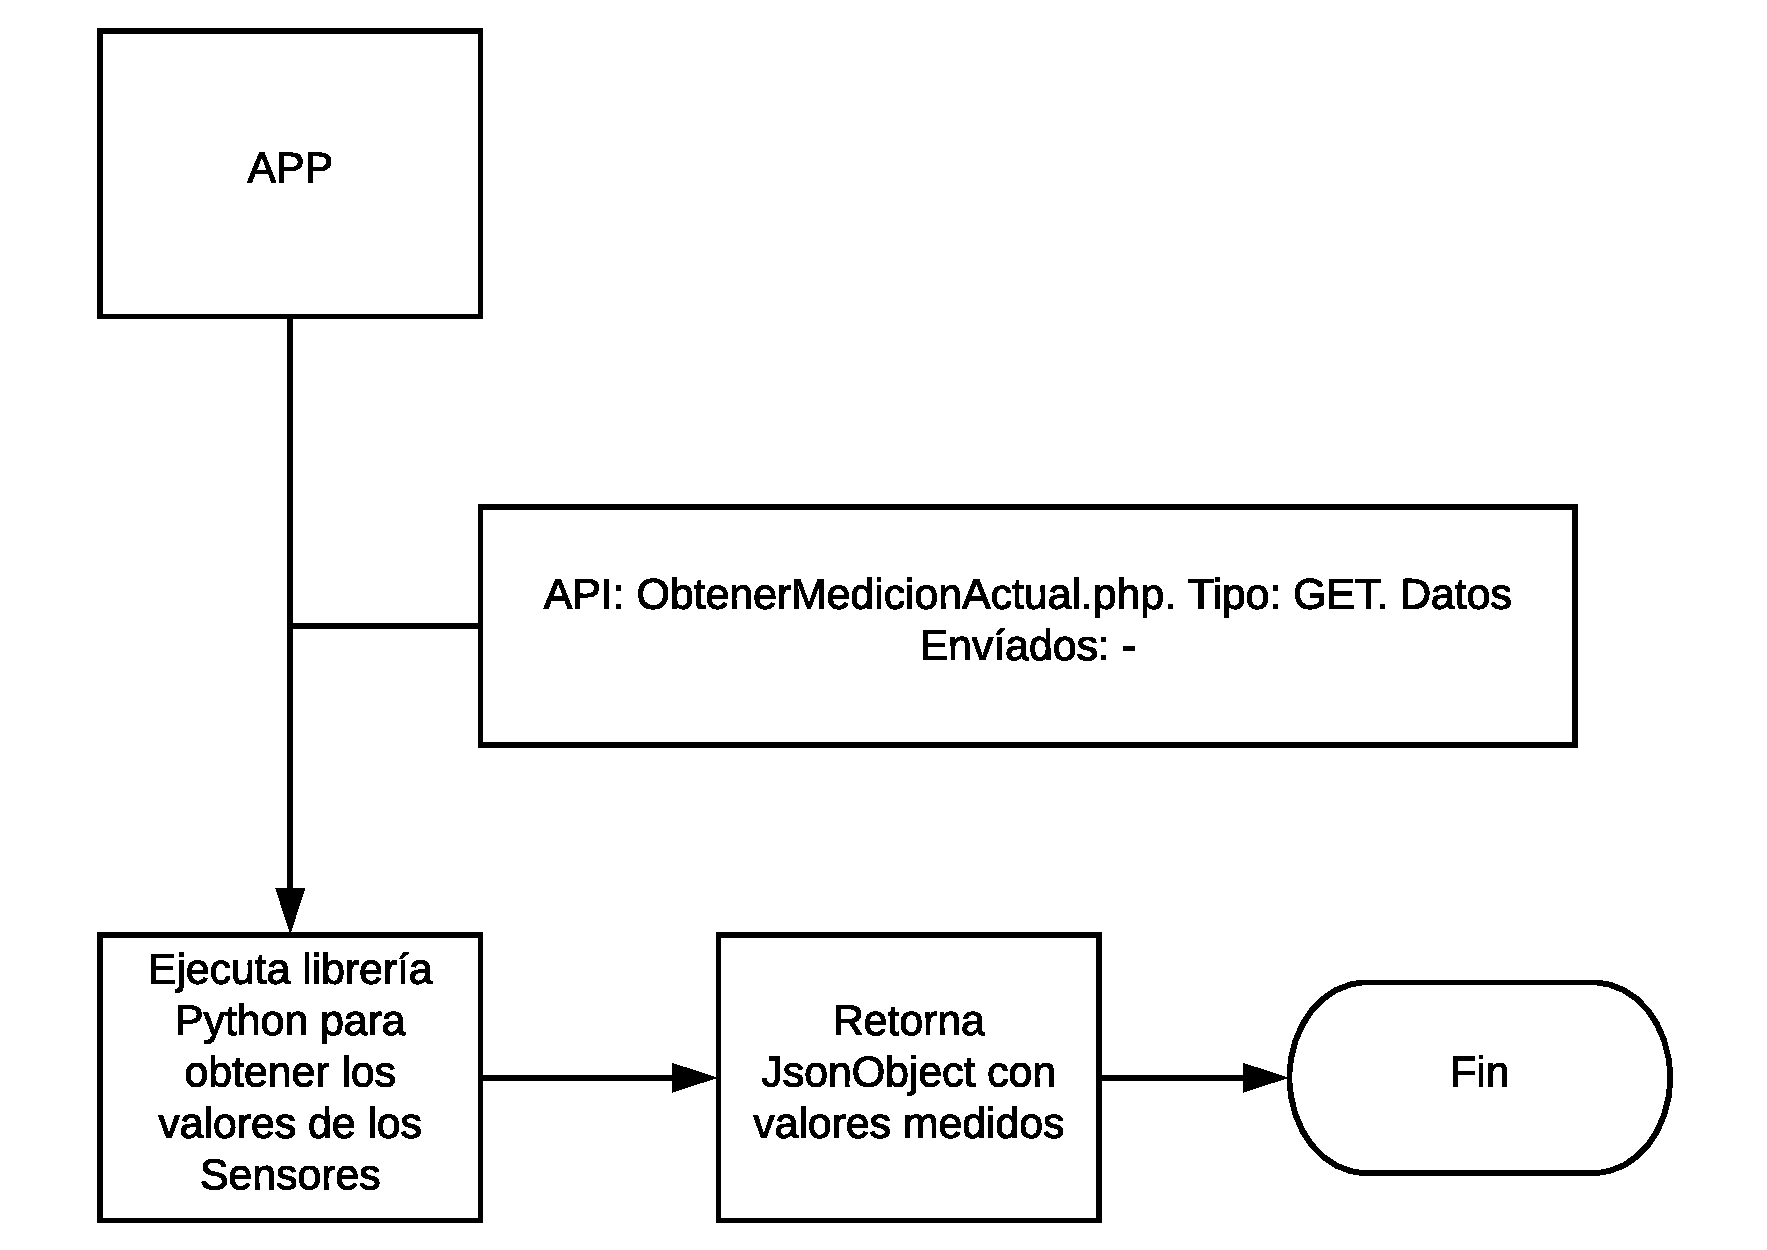
\includegraphics[scale=0.40]{DiagramaGetTempPh.pdf}
                \caption{Diagrama de flujo de obtención de datos de sensores}
                \label{fig:ApiGetTempPh}
            \end{figure}
        
        \subsection{Eliminación experimento de maceración}
        \par En la Figura \ref{fig:ApiRemoveExp}, se presenta el diagrama correspondiente a la API ``\textit{EliminarExp.php}''. Esta es responsable de la eliminación de un experimento en la base de datos de la estación de recolección.
            \begin{figure}[h]
                \centering
                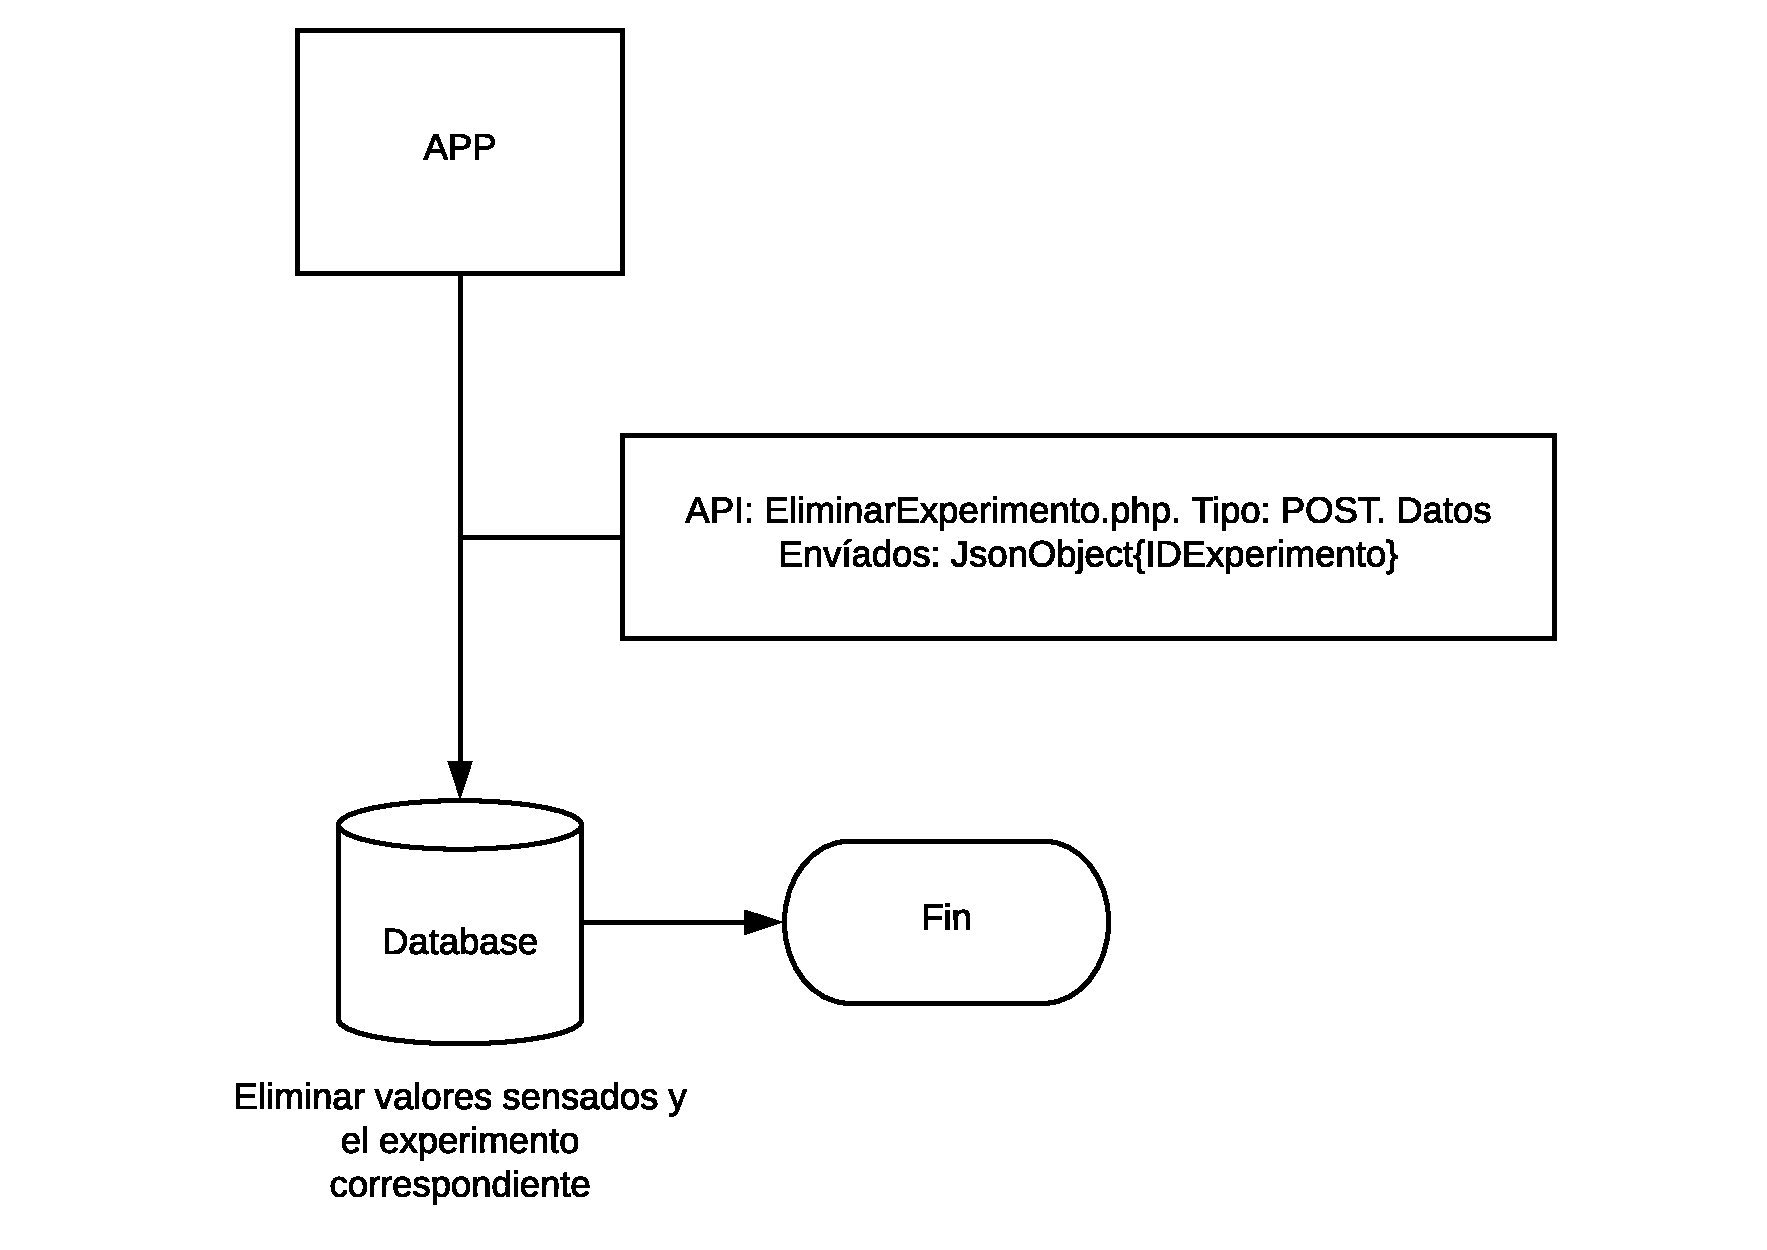
\includegraphics[scale=1]{DiagramaRemoveExp.pdf}
                \caption{Diagrama de flujo de eliminación de experimento}
                \label{fig:ApiRemoveExp}
            \end{figure}
            
        \subsection{Cancelación experimento de maceración}
            \par En la Figura \ref{fig:ApiCancelExp} se presenta el diagrama correspondiente a la API ``\textit{CancelarExp.php}''. Esta es responsable de la cancelación y eliminación de un experimento mientras el mismo se esta llevando a cabo.
            
            
            \begin{figure}[htbp]
                \centering
                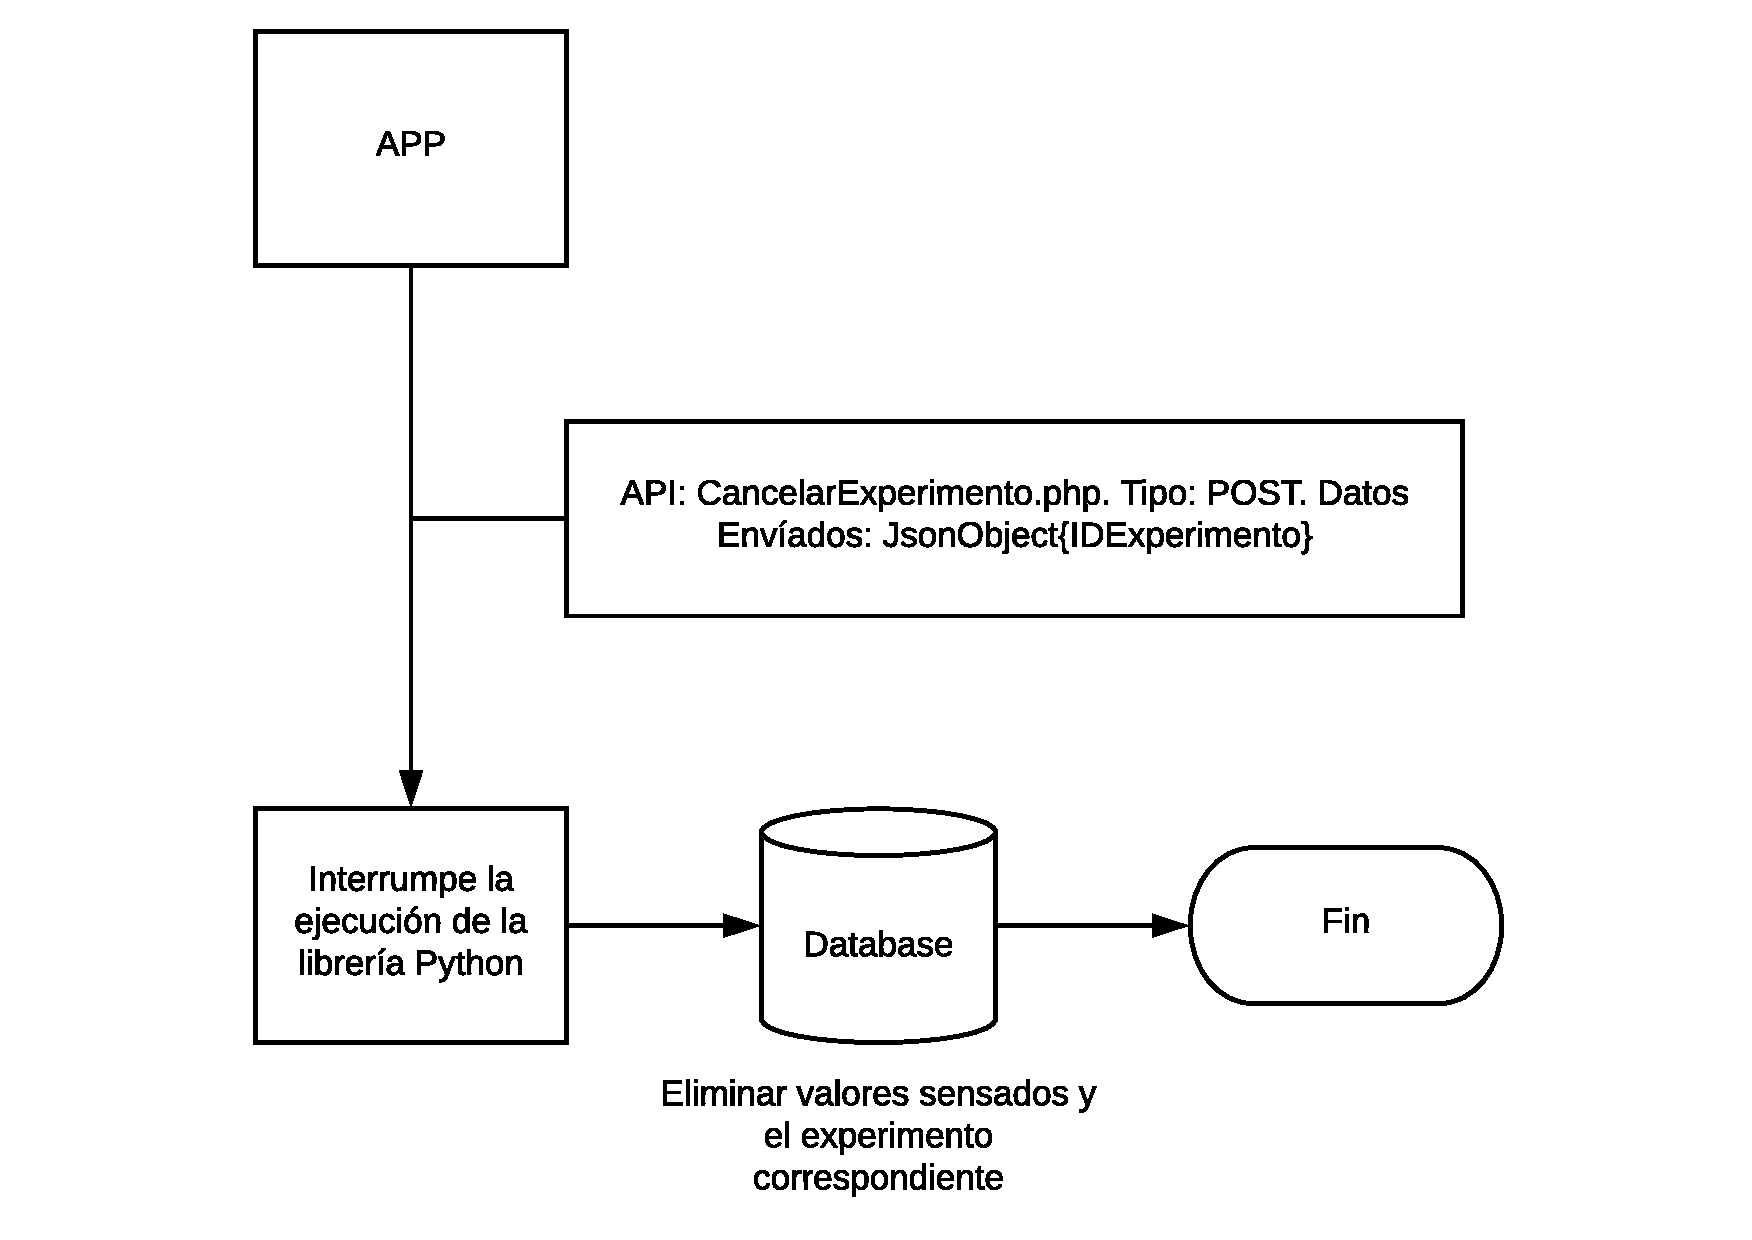
\includegraphics[scale=0.5]{DiagramaCancelExp.pdf}
                \caption{Diagrama de flujo de cancelación de experimento en curso}
                \label{fig:ApiCancelExp}
            \end{figure} \null \vfill
            %\vspace{128cm}
        